%-------------------------------------------------------------------------------------------------------
%-------------------------------------------------------------------------------------------------------
% Sec & Label

\section{Theoretical Analysis}
\label{sec:analysis}


%-------------------------------------------------------------------------------------------------------
%-------------------------------------------------------------------------------------------------------
% Intro

In this section, the circuit in Figure \ref{fig:Desenho_t3} is analysed theoretically.

To begin, the optimization of the values for each component is presented. Afterwards,
the theoretical analysis with those results is shown, with all the plots and tables.


%-----------------------------------------------------------------------
%-----------------------------------------------------------------------
% 		     	    Optim - subsec
% ----------------------------------------------------------------------
% ----------------------------------------------------------------------

\subsection{Optimization}
\label{subsec:optim}

As a consequence of not being given any values, the group had to optimize the values
for each component in order to obtain tha highest Merit possible. Thus, an Octave script
was written to give us the optimal values.


%-----------------------------------------------------------------------
%-----------------------------------------------------------------------
% 			     Results - subsec
% ----------------------------------------------------------------------
% ----------------------------------------------------------------------

\subsection{Theoretical Results}
\label{subsec:res_the}

\begin{figure}[ht]
	\centering
	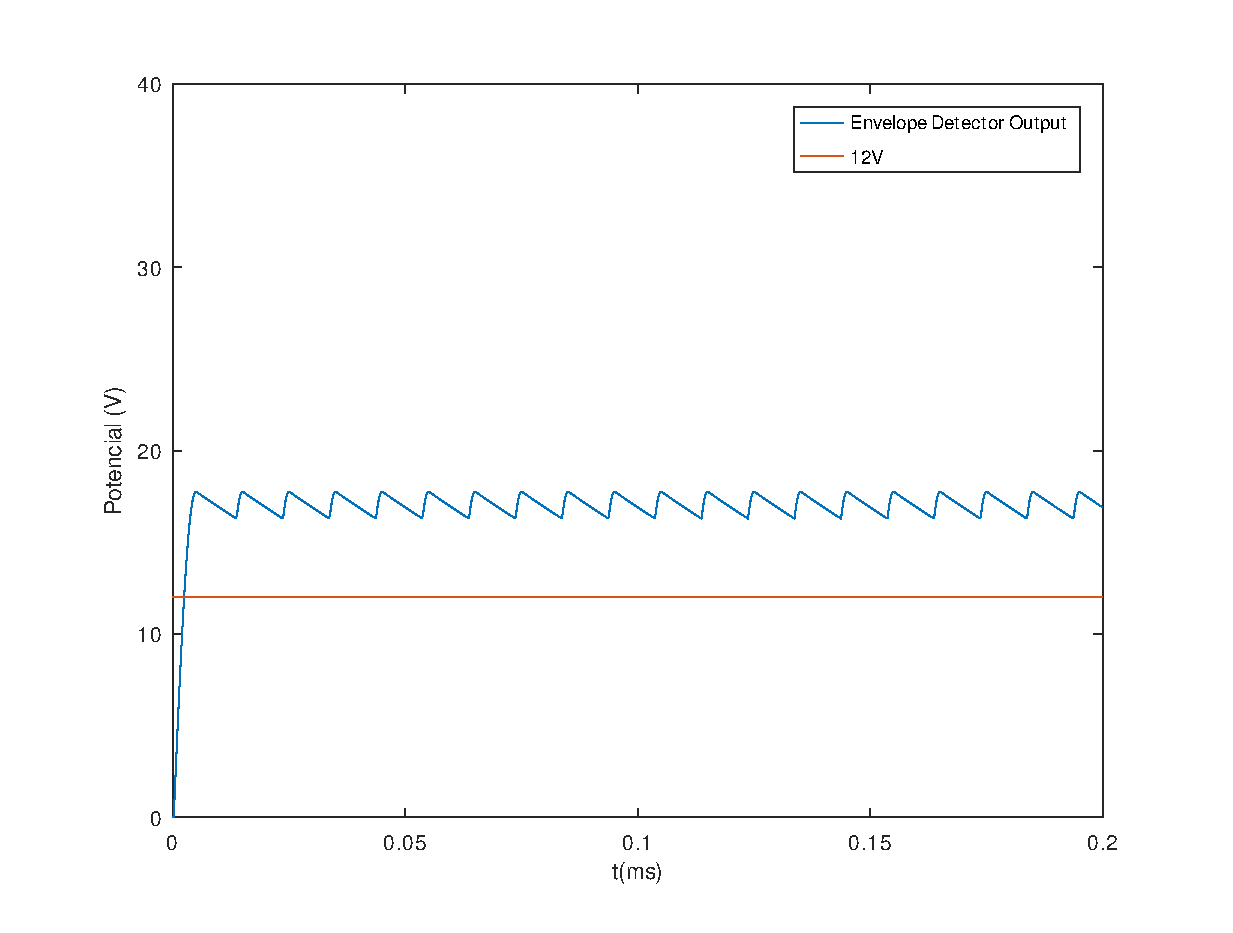
\includegraphics[width=1\linewidth]{envelope_detector.eps}
	\caption{Envelope Detector Circuit $v_{out}$}
\label{fig:EV_vout_a}
\end{figure}

\begin{figure}[ht]
	\centering
	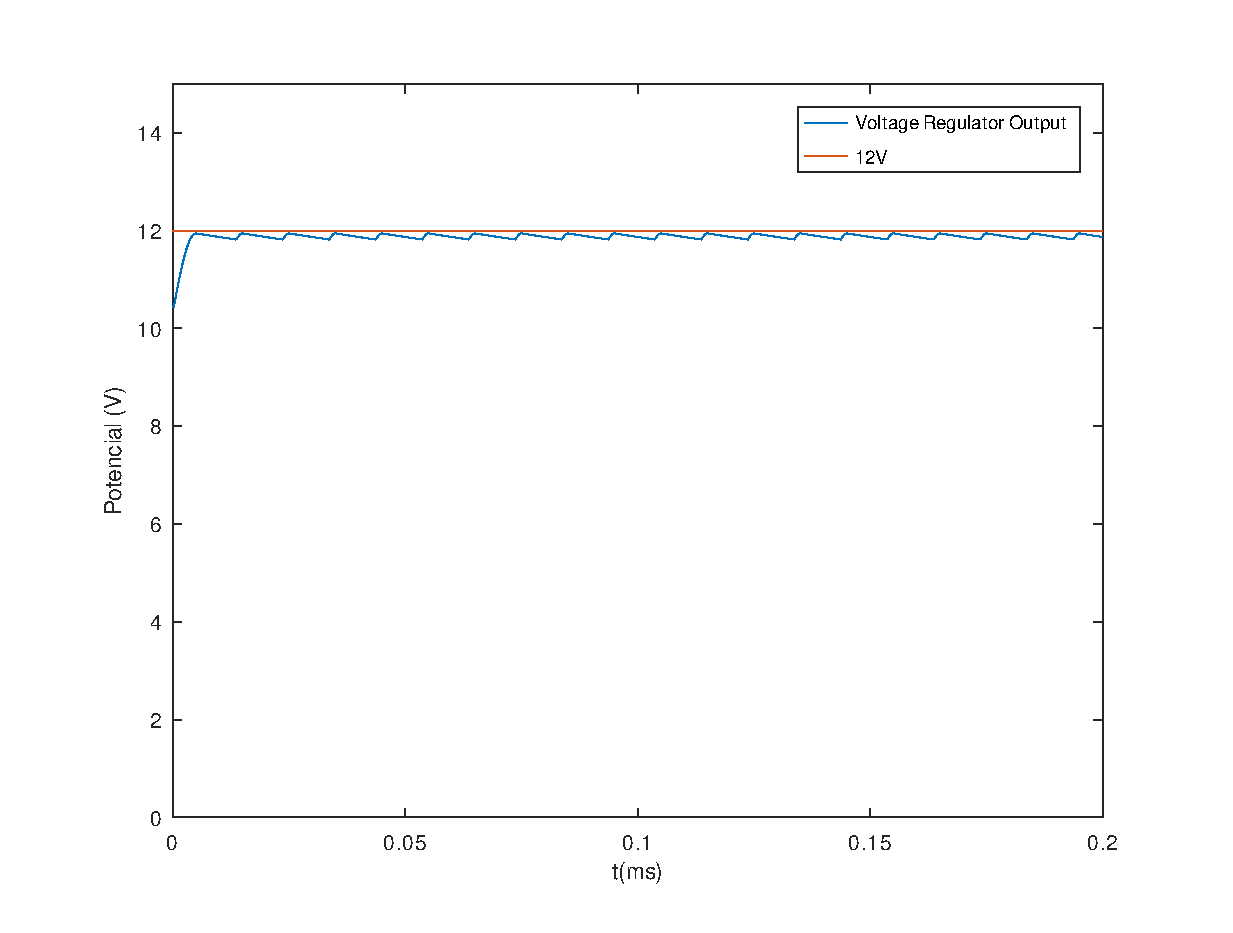
\includegraphics[width=1\linewidth]{voltage_regulator.eps}
	\caption{Voltage Regulator Circuit $v_{out}$}
\label{fig:VR_vout_a}
\end{figure}

